\documentclass[border=8pt]{standalone}
\usepackage{tikz}
\usetikzlibrary{arrows.meta,positioning,calc}
\definecolor{cblue}{RGB}{72,116,158}
\definecolor{cgreen}{RGB}{86,156,104}
\definecolor{corange}{RGB}{214,133,55}
\definecolor{cgray}{RGB}{245,245,245}
\begin{document}
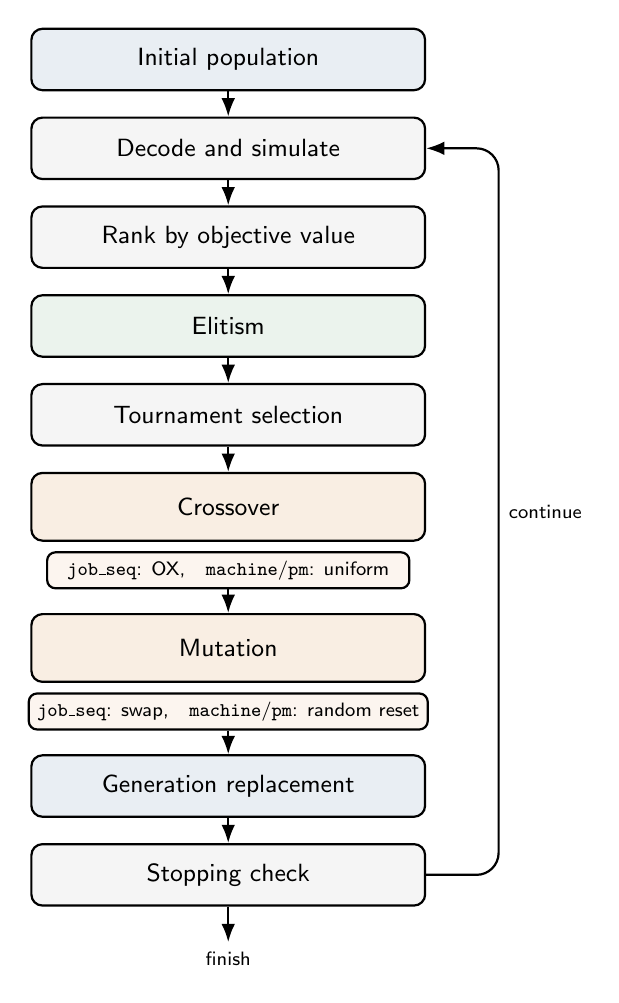
\begin{tikzpicture}[
  font=\sffamily\small,
  >=Latex,
  gastep/.style={draw,thick,rounded corners=4pt,minimum width=5.0cm,minimum height=0.78cm,align=center,inner sep=4pt},
  op/.style={draw,thick,rounded corners=4pt,minimum width=5.0cm,minimum height=0.86cm,align=center,inner sep=4pt},
  note/.style={draw,thick,rounded corners=3pt,minimum width=4.6cm,align=center,inner sep=3pt,font=\sffamily\scriptsize},
  arrow/.style={->,thick},
  loop/.style={->,thick,rounded corners=8pt}
]
  \node[gastep,fill=cblue!12] (init) {Initial population};
  \node[gastep,fill=cgray,below=0.32cm of init] (eval) {Decode and simulate};
  \node[gastep,fill=cgray,below=0.32cm of eval] (rank) {Rank by objective value};
  \node[gastep,fill=cgreen!12,below=0.32cm of rank] (elite) {Elitism};
  \node[gastep,fill=cgray,below=0.32cm of elite] (select) {Tournament selection};
  \node[op,fill=corange!14,below=0.32cm of select] (cross) {Crossover};
  \node[note,fill=corange!8,below=0.12cm of cross] (crossnote)
    {\texttt{job\_seq}: OX,\quad \texttt{machine}/\texttt{pm}: uniform};
  \node[op,fill=corange!14,below=0.30cm of crossnote] (mut) {Mutation};
  \node[note,fill=corange!8,below=0.12cm of mut] (mutnote)
    {\texttt{job\_seq}: swap,\quad \texttt{machine}/\texttt{pm}: random reset};
  \node[gastep,fill=cblue!12,below=0.30cm of mutnote] (replace) {Generation replacement};
  \node[gastep,fill=cgray,below=0.32cm of replace] (stop) {Stopping check};

  \draw[arrow] (init) -- (eval);
  \draw[arrow] (eval) -- (rank);
  \draw[arrow] (rank) -- (elite);
  \draw[arrow] (elite) -- (select);
  \draw[arrow] (select) -- (cross);
  \draw[arrow] (crossnote) -- (mut);
  \draw[arrow] (mutnote) -- (replace);
  \draw[arrow] (replace) -- (stop);
  \draw[loop] (stop.east) -- ++(0.92,0) |- node[pos=0.25,right,font=\sffamily\scriptsize] {continue} (eval.east);
  \draw[arrow] (stop.south) -- ++(0,-0.45) node[below,font=\sffamily\scriptsize] {finish};
\end{tikzpicture}
\end{document}
